
\ifintegriereaufgaben

\section*{Stabilit�t und Eigenl�sungen Aufgaben}\label{MA2-stabilitaet-aufgaben}
Regeln und Beispiele, die zur Bearbeitung der Aufgaben hilfreich sind, finden Sie im Skript\wennreferenzvorhanden{MA2-stabilitaet}{ (Abschnitt \abschnittsverweis{MA2-stabilitaet})}.
\else
\section{Stabilit�t und Eigenl�sungen Aufgaben}\label{MA2-stabilitaet-aufgaben}

Regeln und Beispiele zu diesen Aufgaben finden Sie im Skript.
\fi
Zu diesen Aufgaben ist noch keine ausgearbeitete L�sungssammlung enthalten.


%\begin{exercisebox}[Stabilit�t] % (beide EW <0 -> asymptotisch stabil)
%Gegeben sei das lineare System
%
%\[
%\dot{x} = Ax, \qquad
%A=
%\begin{pmatrix}
%-2 & 1 \\
%0 & -3
%\end{pmatrix}.
%\]
%
%\begin{enumerate}
%\item Bestimmen Sie die Eigenwerte von \(A\).
%\item Untersuchen Sie die Stabilit�t des Gleichgewichtspunktes \(x=0\).
%\item Skizzieren Sie qualitativ das Verhalten der L�sung f�r \(t\to\infty\).
%\end{enumerate}
%\end{exercisebox}

\begin{exercisebox}[Stabilit�t] %  (EW 2 > 0 -> instabil)
Gegeben sei

\[
A=
\begin{pmatrix}
2 & 0 \\
0 & -1
\end{pmatrix}.
\]

\begin{enumerate}
\item Bestimmen Sie die Eigenwerte.
\item Ist das System, das durch \(A\) beschrieben wird, stabil?
\item Welche Richtung w�chst exponentiell?
\end{enumerate}

\end{exercisebox}

\begin{exercisebox}[Stabilit�t] %  (negativer Realteil -> stabile Spirale
Das System

\[
\dot{x} =
\begin{pmatrix}
0 & 1 \\
-4 & -1
\end{pmatrix}
x
\]

beschreibt einen ged�mpften Oszillator.

\begin{enumerate}
\item Bestimmen Sie die Eigenwerte.
\item Welche Art von Stabilit�t liegt vor?
\end{enumerate}

\end{exercisebox}

\begin{exercisebox}[Stabilit�t]
Ein elektrisches System wird beschrieben durch

\[
\dot{x} =
\begin{pmatrix}
-1 & 2 \\
0 & -3
\end{pmatrix}
x.
\]

\begin{enumerate}
\item Bestimmen Sie die Eigenwerte.
\item Ist das System stabil?
\item Was bedeutet das f�r das elektrische Netzwerk?

\end{enumerate}
\end{exercisebox}

%\begin{exercisebox}[Stabilit�t (Kriterium)]
%Die Polstellen eines Systems sind
%
%\[
%s=-2 \pm 3\,i\,.
%\]
%
%Welche Aussage ist korrekt?
%
%\begin{itemize}[label={$\Box$}]
%\item Das System zeigt eine ged�mpfte Schwingung.
%\item Das System w�chst exponentiell.
%\item Das System ist konstant.
%\item Das System ist instabil.
%\end{itemize}
%\end{exercisebox}

\begin{exercisebox}[Stabilit�t (Kriterium)]
Gegeben sei

\[
A=
\begin{pmatrix}
a & b \\
c & d
\end{pmatrix}.
\]

\begin{enumerate}
\item Zeigen Sie, dass

\[
\lambda^2-(a+d)\lambda+(ad-bc)=0
\]

das charakteristische Polynom ist.

\item Welche Bedingungen an Spur und Determinante garantieren Stabilit�t?
\end{enumerate}
\end{exercisebox}

	\begin{exercisebox}[Stabilit�t (Kriterium)]
Die folgende Skizze zeigt eine ged�mpfte Schwingung.

\begin{center}
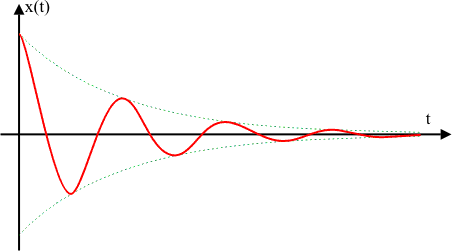
\includegraphics[width=6cm]{../Mathematik_2/Bilder/federpendel_gedaempfte_schwingung_zeitverlauf.png}
\end{center}
\begin{enumerate}

\item Welche Form hat die zugrunde liegende Funktion?
\item Welche Rolle spielen Real- und Imagin�rteil des Exponenten?

\end{enumerate}
\end{exercisebox}

%\begin{exercisebox}[Stabilit�t (Kriterium)]
%Ein lineares System
%
%\[
%\dot{x}=A\,x
%\]
%
%besitzt Eigenwerte
%
%\[
%\lambda_1=-2, \qquad \lambda_2=-1.
%\]
%
%Welche Aussage ist korrekt?
%
%\begin{itemize}[label={$\Box$}]
%\item Das System ist asymptotisch stabil.
%\item Das System ist instabil.
%\item Das System besitzt periodische L�sungen.
%\item Das System divergiert.
%\end{itemize}

%\end{exercisebox}

%\begin{exercisebox}[Stabilit�t (Eigenwerte)]
%Gegeben sei
%
%\[
%A=
%\begin{pmatrix}
%-2 & 1 \\
%0 & -3
%\end{pmatrix}.
%\]
%
%\begin{enumerate}
%
%\item Bestimmen Sie die Eigenwerte.
%\item Ist das System stabil?
%
%\end{enumerate}
%\end{exercisebox}
%
%
%\begin{exercisebox}[Stabilit�t (Phasenportrait)]
%Das System
%
%\[
%\dot{x}=
%\begin{pmatrix}
%0 & 1 \\
%-1 & 0
%\end{pmatrix}x
%\]
%
%beschreibt eine Bewegung.
%
%\begin{enumerate}
%\item Bestimmen Sie die Eigenwerte.
%\item Welche Art von Stabilit�t liegt vor?
%\item Skizzieren Sie das Phasenportrait.
%\end{enumerate}
%\end{exercisebox}
